\chapter{Einleitung}
%Motivation
%%Umfeld
%Problemstellung
%Ziel
%%Herangehensweise
%%Verwandte Arbeiten
%%Konkrete Ziel
%Stuktur der Arbeit

\section{Motivation}
%%Umfeld
Eine 2017 veröffentlichte Statistik zeigt, wie stark die Akzeptanz von intelligenten Geräten zwischen 2015 und 2017 angestiegen ist: während bei smarten Thermostaten mit einem Prozent der geringste Anstieg zu verzeichnen war, stieg sie bei Fitness-Trackern um mehr als das Dreifache \cite{nier_2017}. Weitemeyer prognostiziert bis 2020 weiterhin einen Anstieg an vernetzten Geräten in Deutschland \cite{weitemeyer_2018}.
Zusammen mit der Akzeptanz sind allerdings in den letzten Jahren ebenfalls die Angriffe von Kriminellen gegen Geräte im sogenannten \ac{IoT}, oder auch \emph{intelligente Geräte} genannt, gestiegen \cite{statista_2019}.

%Warum (Fallbeispiele) 
Darüber hinaus finden sich solche Fälle von Angriffen oder Verstößen gegen die Privatsphäre immer häufiger in den Medien \cite{holland_2016,it_verlag_informationstechnik_gmbh_2018}. Aus diesem Grund beschäftigen sich auch Unternehmen im IT-Sicherheitssektor mit diesen Themen und untersuchen verschiedene Produkte auf ihre Anfälligkeit für solche Attacken bzw. deren Schwachstellen \cite{lorenz_2018,ao_kaspersky_lab_2018}.

Beispielsweise untersuchte das Unternehmen \emph{Positive Technologies} einen intelligenten Saugroboter \cite{salmi_2017}.
Dieser enthielt zwei kritische Schwachstellen, mithilfe derer ein Angreifer nicht nur Informationen von dem Roboter bekommen konnte, sondern ihn Befehle ausführen lassen und somit die vorhandene Kamera mit einer Nachtsichtfunktion ansteuern konnte. Die Konsequenz war, dass der Angreifer ein aktuelles Kamerabild sowie Zugriff auf das Netzwerk hatte, in dem sich der Roboter befand. Die Tatsache, dass die Schwachstelle in einem, durch eine Anmeldung geschützten Bereich war, hinderte nicht, da die Standardpasswörter der Produkte oft nicht geändert werden \cite{positive_technologies_2018}.
Auch deckt sich dies mit den Top 10 Risiken 2018 des \ac{OWASP}, bei der die drei größten Schwachstellen aus den folgenden Kategorien kommen: \emph{Weak Guessable, or Hardcoded Passwords}, \emph{Insecure Netzwerk Services} und \emph{Insecure Ecosystem Interfaces}. Dies bestätigen auch weiteren Artikeln \cite{guzman_2019,eckstein_2018}.
Diese Aussage bestätigen auch zwei Berichte aus 2014 und 2018.
Im Jahr 2014 schrieb Trustwave \cite{trustwave_holdings_inc_2014}: \emph{Thirty percent of the time, an attacker gains access because of a weak password.}
Vergleicht man dies mit dem aktuellsten Global Security Report 2018, wird erkenntlich, dass die Anzahl dieser Fälle abgenommen hat, allerdings immer noch die zweithäufigste Schwachstelle ist \cite{trustwave_holdings_inc_2018}.

\section{Problemstellung}
%%Problemstellung
    Um das Gerät sowie den vom Betreiber zur Verfügung gestellten Dienst auf Schwachstellen untersuchen zu können, ist es notwendig, sich mit dem zur Kommunikation genutzten Protokoll auseinander zu setzen. Dazu gehört beispielsweise darüber gesendete Nachrichten zu bearbeiten und erneut zu senden oder neue Nachrichten im Namen des eigentlichen Gerätes zu verfassen. Damit wird versucht, dass IT-Schutzziel Authentizität zu umgehen \cite{Bedner2010}.
        
    Um solche Schwachstellen in Geräten, herstellerübergreifend erkennen zu können, wird ein Tool benötigt, dass die Kommunikation abfangen und manipulieren kann.

\section{Ziel der Arbeit}
%Forschungsfrage!
    In der Arbeit wird untersucht, ob es möglich ist, mithilfe eines Programms die übertragenen Daten der intelligenten Geräte herstellerübergreifend abzufangen und verändern zu können.

%%Herangehensweise
    Um diese Fragestellung zu beantworten, wird ein Konzept entworfen, welches mithilfe eines Proxies in der Lage sein soll, die gewünschte Verbindung zu verändern. Es wird versucht eine möglichst zuverlässige Weiterleitung der Pakete ermöglichen um die Lösung praktikabel zu machen.
    
\section{Existierende Lösungen}
%Implementierungen auf dem Markt
    Folgende Implementierungen wurden bereits entwickelt, die das Ziel haben, Nachrichten des \ac{MQTT}-Protokolls an ein drittes Gerät weiterzuleiten.
    %Diese sind interessant, da diese Funktionalität im Standard \cite{gupta_banks_2015} nicht unterstützt wird. Durch das Publish/Subscribe-Prinzip ist der Broker nicht in der Lage, selbst kommunizieren zu können. Er kommuniziert ausschließlich die neuen Nachrichten an die abonnierenden Geräte weiter und kann nicht selbst Nachrichten schicken.
    
    \subsection{MQTT Bridges}
        Entwickler mehrerer MQTT-Bibliotheken haben erkannt, dass die Funktionalität für das Weiterleiten von Nachrichten an weitere Geräte in gewissen Anwendungsfällen sehr hilfreich sein kann \cite{84codes_ab_2016,light_2019}. Beispielsweise wird diese Funktionalität benötigt, um Geräte, welche \ac{MQTT} für die Kommunikation nutzen, mit anderen Geräten sprechen zu lassen und somit von dem Status abhängige Abläufe zu ermöglichen.
        Um dieses Problem zu lösen, wurden diese Bibliotheken um die MQTT-Bridge-Funktionalität erweitert. Sie besteht aus einem Client, der an den Broker angeschlossen wird. Mithilfe von modifizierten Ereignissen, die aktiviert werden sobald der Broker eine Nachricht empfängt, können die Nachrichten direkt an einen zusätzlichen Client weitergeleitet werden, der sich mit einem weiteren Broker verbunden hat.
    
    \subsection{Axway - API Management Plus}
        Die API-Management-Software von Axway vereint das Erstellen und Organisieren vieler verschiedener Schnittstellen mit direkten Anbindungsmöglichkeiten für Endgeräte. Darüber hinaus können alle Endpunkte auf fehlerhaftes Verhalten oder Anfragen geprüft werden. Dies soll ermöglichen, auf schnelle Änderungen des Marktes einzugehen und viele verschiedene Geräte parallel zu unterstützen.
        Um auch intelligente Geräte aus dem \ac{IoT}-Bereich unterstützen zu können, wurde ein Proxy für das \ac{MQTT}-Protokoll entwickelt \cite{axway_2018}. Der Proxy befindet sich zwischen dem Client und dem Broker. Dadurch hat er die Möglichkeit, die eingehenden Pakete abzufangen und anhand eines Regelwerks, welches per \ac{REST}\footnote{Ist ein Architekturstiel der helfen soll verteilte Anwendungen zu realisieren und zu organisieren. Es ist kein Regelwerk und besitzt somit auch keine Regeln oder Standards die eingehalten werden müssen. \cite{Doglio2015}} über den \acs{API}-Manager erreichbar ist, Daten zu validieren.
        
        Das Ziel dieser Lösung ist somit, auf Basis der Richtlinien, welche auf dem Mana-gement-Server hinterlegt werden, gesendete Nachrichten des \ac{MQTT}-Protokolls zu filtern und nicht regelkonforme Kommunikation zu blockieren. Dies ermöglicht, mithilfe eines Identifizierungsmerkmals, Beispielsweise Zugriffe auf Topics oder das Versenden von Nachrichten einzuschränken..
        
        Die Lösung wird in verschiedenen Versionen als Docker-Container bereitgestellt. Für den Fall, dass bereits ein eigener Broker und ein Regelwerk im Einsatz sind, kann der \ac{MQTT}-Proxy alleinstehend betrieben werden. Falls jedoch alle Systeme benötigt werden, können Broker, Regelwerk und Proxy auf einmal aufgesetzt werden, um eine direkte Testumgebung bereitzustellen.
        
        Jedoch besitzt diese Lösung gewisse Einschränkungen.
        Es ist zum Beispiel nicht möglich, mehrere Broker per Proxy-Instanz zu definieren oder \acs{TLS}-Unterstützung zwischen Client und Proxy sowie Proxy und Broker zu ermöglichen.
        Trotz den Einschränkungen ist es möglich, bei einer unverschlüsselten Kommunikation Daten abzufangen, deren Inhalt auszuwerten und anhand von Regeln Pakete zu verwerfen.
        
        Der Datenfluss sieht wie folgt aus.
        \begin{figure}[h]%h=direkt danach t=top b=bottom
            \centering
            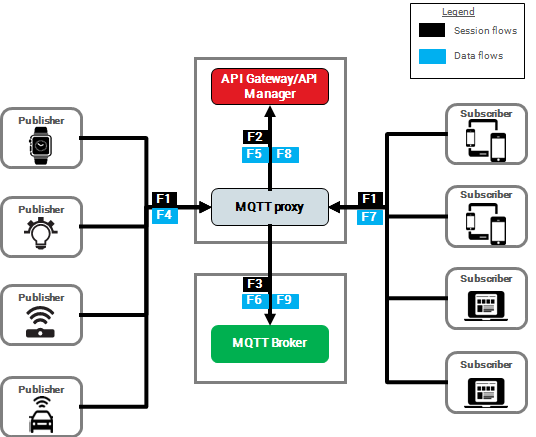
\includegraphics[width=14cm]{tex/bilder/2_grundlagen/axway-mqtt-proxy02_short.png}
            \captionof{figure}{Datenfluss des Axway MQTT-Proxys \cite{axway_2018}}
            \label{fig:axway-proxy}
        \end{figure}
        \begin{itemize}
            \item F1: Das \ac{IoT}-Gerät (auch \emph{Client} genannt) sendet eine \emph{Connect-Nachricht} mit Benutzerdaten zum Proxy, um sich mit diesem zu verbinden
            \item F2: Die Benutzerdaten werden zum Verifizieren dem API-Gateway gesendet
            \item F3: Mit der Bestätigung vom Gateway wird die Sitzung zum Proxy hergestellt
            \item F4: Das Gerät sendet eine Nachricht an den Proxy
            \item F5: Der Proxy verifiziert und ändert gegebenfalls die Nachricht auf Basis der Gateway-Regeln
            \item F6: Die Nachricht wird an den externen Broker weitergeleitet
            \item F7: Um nun eine Antwort zu erhalten, sendet der Client eine \emph{Subscribe-Nachricht} an den Proxy
            \item F8: Der Proxy verifiziert und ändert gegebenfalls die Nachricht auf Basis der Gateway-Regeln
            \item F9: Der Proxy leitet die Nachricht an den externen Broker weiter
        \end{itemize}
    %Analyse der Lösung
    Diese Implementierungen besitzen bereits die Möglichkeit, Daten weiterzuleiten und den Inhalt auszuwerten. Jedoch fehlen folgende Inhalte:
    \begin{itemize}
        \item Schnittstelle zum senden selbst erzeugter Nachrichten an das gewählte Ziel.
        \item Erneutes Versenden von bereits gesendeten Nachrichten um Nebeneffekte oder zustandsabhängige Funktionen zu erkennen.
        \item Manuelle Manipulation der ausgehenden und ankommende Pakete.
    \end{itemize}
    
    Diese Punkte werden in dieser Arbeit mit berücksichtigt um diese 

\section{Struktur der Arbeit}
%Struktur
    In Kapitel \ref{MQTT} dieser Arbeit wird Wissen über die benötigten, grundlegende Protokoll vermittelt.
    Anschließend werden in Kapitel \ref{TechKonzepte} die darauf aufbauenden Konzepte erläutert und in den Kontext der Forschungsfrage gestellt.
    %Nachdem die Grundlagen vermittelt wurden, bekommt der Leser eine Übersicht über bereits vorhandene Konzepte und Herangehensweisen zur Absicherung von \ac{IoT} oder im deutschen Sprachgebrauch \emph{Internet der Dinge}. 
    Dies soll den Leser befähigen, die vorgestellten Produkte sowie die Entwicklung und Umsetzung des in dieser Arbeit erstellten Konzepts korrekt einordnen und bewerten zu können.
    Direkt im Anschluss wird das Konzept der eigenen Software erläutert und auf Schwierigkeiten sowie deren Lösungen eingegangen. Das darauf folgende Kapitel \emph{Implementierung des Prototypen} beschreibt die Umsetzung des zuvor erläuterten Konzepts und setzt die Rahmenbedingungen und verwendeten Technologien fest. Um die Ergebnisse der Arbeit bewerten zu können, wird im Anschluss eine Validierung anhand von Versuchen durchgeführt und die Ergebnisse der Forschungsfrage festgehalten. Zuletzt wird ein Ausblick gegeben, welche Probleme, Gefahren und Potenziale sich in Zukunft ergeben könnten und welche weiteren Arbeiten sich zu diesen Themen anbieten.